\chapter{What you did}
\label{ch:whatYouDid}


% \engExpl{Choose your own chapter title to describe this}
% \sweExpl{[Vad gjorde du? Hur gick det till? – Välj lämplig rubrik (“Genomförande”, “Konstruktion”, ”Utveckling”  eller annat]}


% \engExpl{What have you done? How did you do it? What design decisions did you make? How did what you did help you to meet your goals?}
% \sweExpl{Vad du har gjort? Hur gjorde du det? Vilka designval gjorde du?\\
% Hur kom det du hjälpte dig att uppnå dina mål?}


% the following sets the TOC entry to break after the & - note you have to include the first letter of the following word as it get swolled by the \texorpdfstring{}{} processing


\section[Hardware/Software design …/Model/Simulation model \&\texorpdfstring{\\}{ p} parameters/…]{Hardware/Software design …/Model/Simulation model \& parameters/…}


\section{Proof of Concepts}


\section{The architecture of the software}


% https://lucid.app/lucidchart/f5dc4477-fa25-44e8-93d9-946def9cd4a9/edit

\begin{figure}[H]
    \centering
    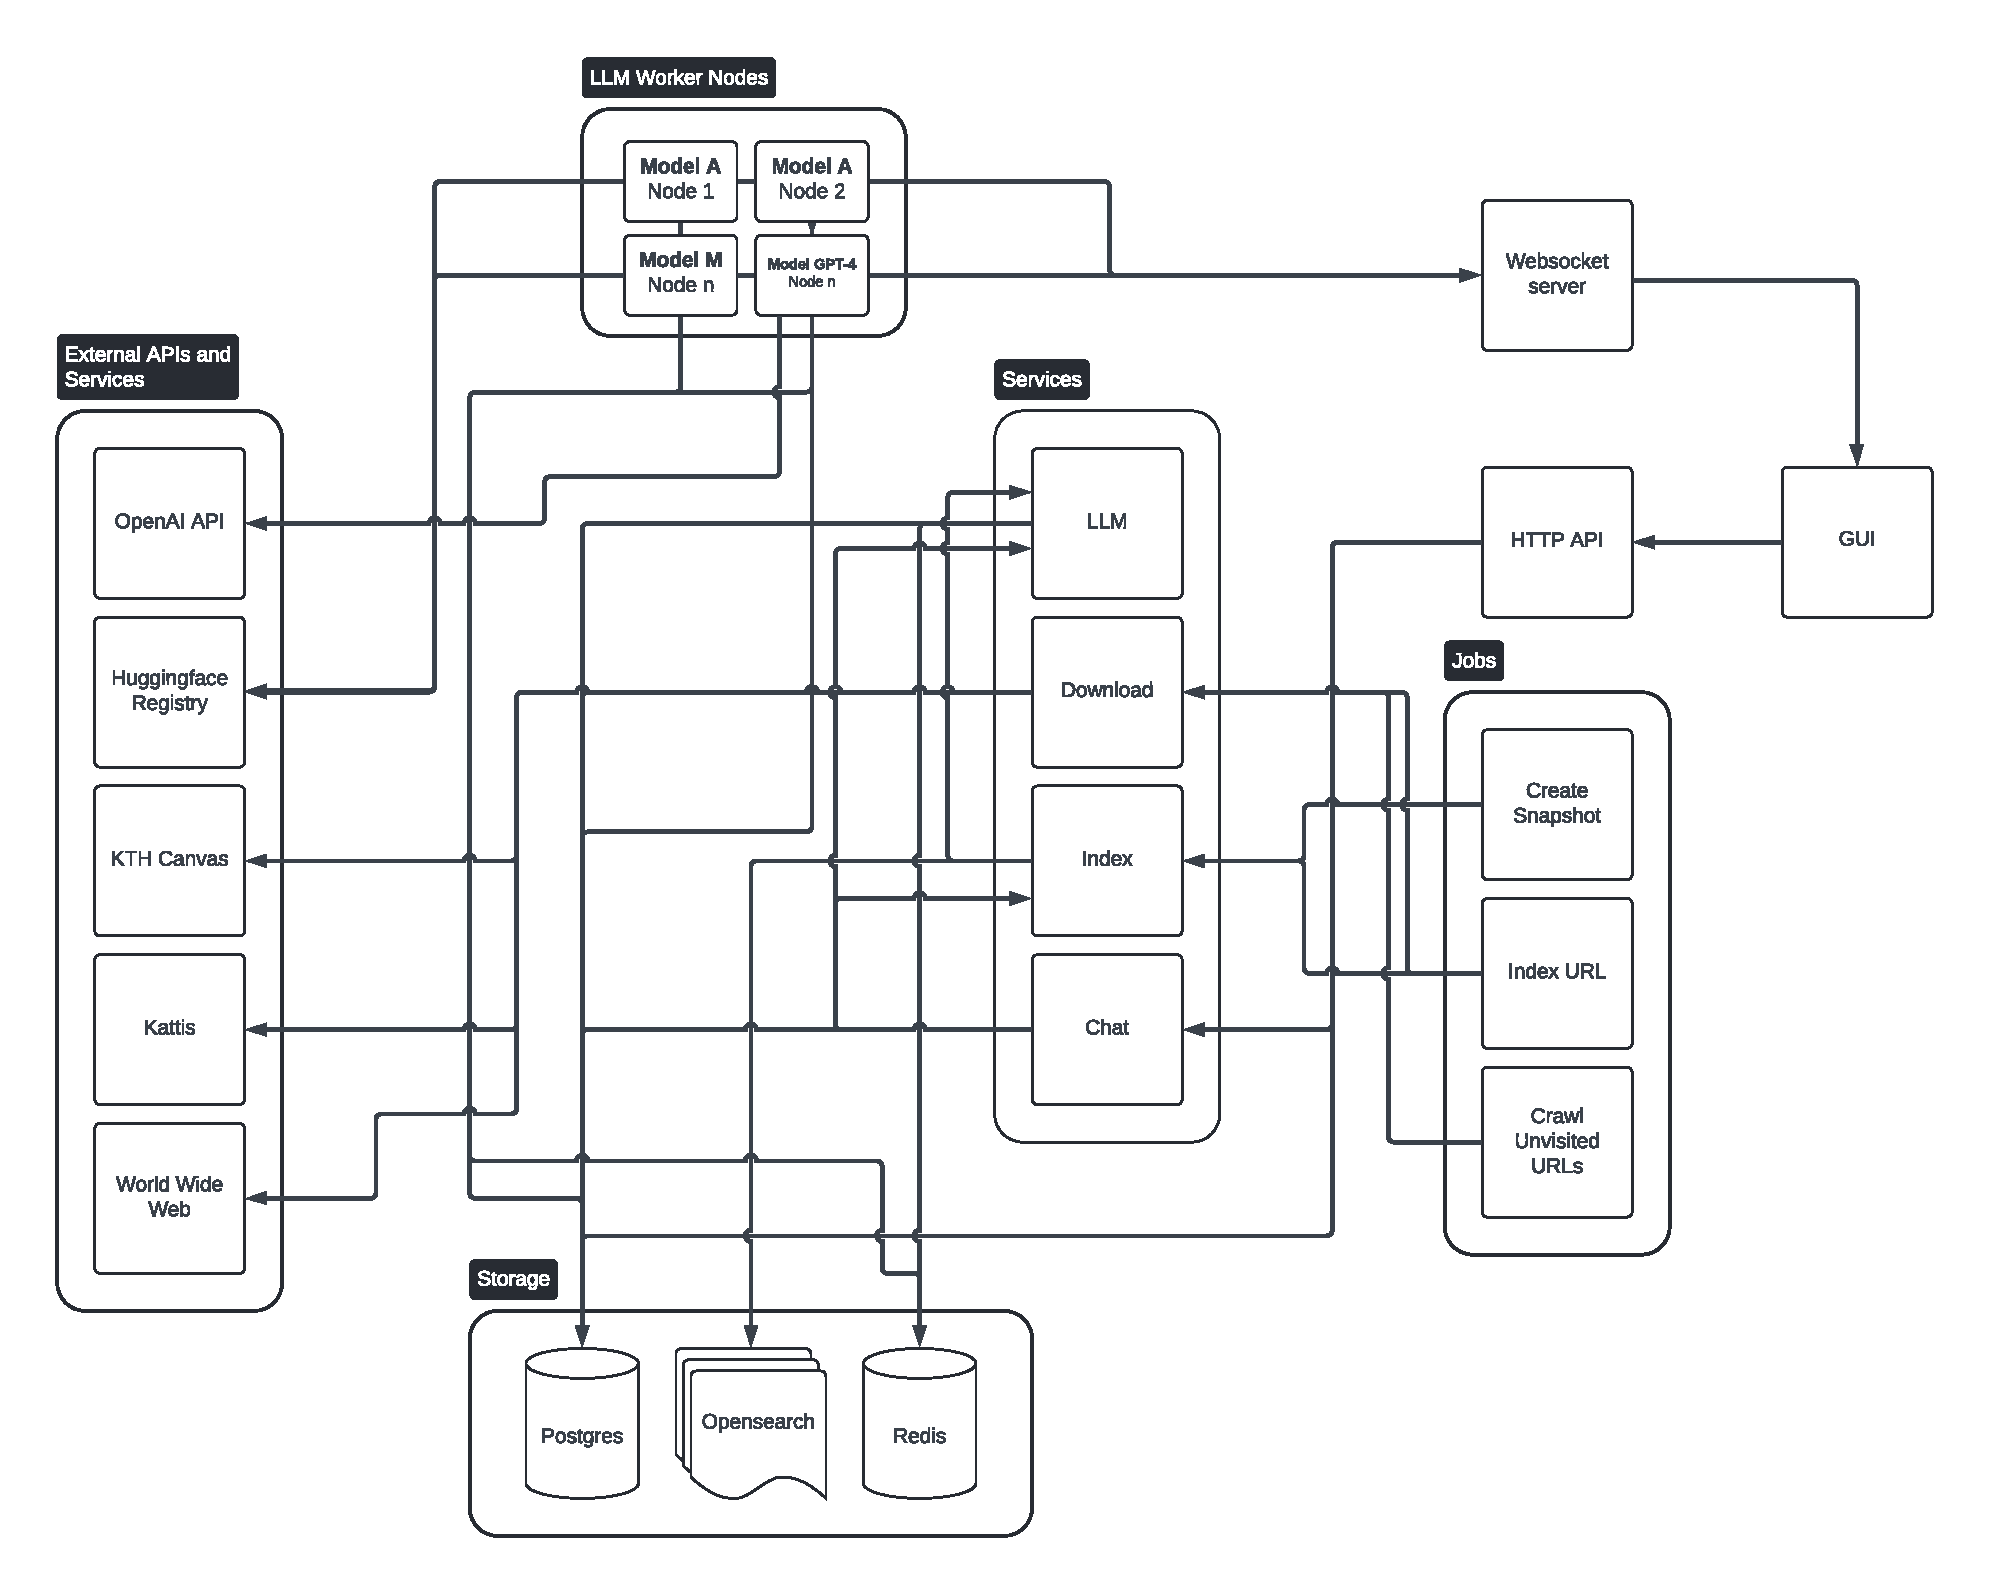
\includegraphics[width=\textwidth]{content/figures/assets/06-system-architecture-diagram.pdf}
    \caption{Diagram that shows the system architecture of the software constructed to run the study}
    \label{fig:system_architecture_diagram}
\end{figure}



\subsection{Courseroom Crawler}


\subsection{Running large language models at scale}


\subsection{Datastore and Index}


\subsection{User interface}


\section{How the software is deployed}


% \sweExpl{Hårdvara / Mjukvarudesign ... / modell / Simuleringsmodell och parametrar / …}




% \sweExpl{Figur~\ref{fig:homepageicon}  visar en enkel ikon för en hemsida. Tiden för att få tillgång till den här sidan när den laddas kommer att kvantifieras i en serie experiment. De konfigurationer som har testats i provbänk listas ini tabell~\ref{tab:configstested}.\\
% Vad du har gjort? Hur gjorde du det? Vilka designval gjorde du?}


\section{Implementation …/Modeling/Simulation/…}
\label{sec:implementationDetails}


\subsection{Some examples of coding}


% \engExpl{This section is simply to show some example of how you can include code in your thesis - this is not a section you would have in your thesis.}
% \sweExpl{Det här avsnittet är helt enkelt för att visa ett exempel på hur du kan inkludera kod i ditt examensarbete - det här är inte ett avsnitt du skulle ha i ditt examensarbete.}


\subsection{Some examples of figures in tikz}


% \engExpl{This section is simply to show some example of how you can draw your own figures for in your thesis - this is not a section you would have in your thesis.}
% \sweExpl{Det här avsnittet är helt enkelt för att visa ett exempel på hur du kan rita dina egna figurer i ditt examensarbete – det här är inte ett avsnitt du skulle ha i ditt examensarbete.}
% These figures are just some examples to show that you can draw your own figures for in your thesis. This has two advantages: \first you do not have to worry about copyrights -- as these are your own figures and \Second the text is now readable and not simply a picture of text -- so screen readers can read the figure's contents to someone who is listening to the contents of your thesis.


\subsubsection{Azure's Form Recognizer}


\cleardoublepage